\documentclass[english,12pt]{article}
\usepackage[T1]{fontenc}
\usepackage{geometry}
\geometry{verbose,bmargin=2.5cm,lmargin=2.5cm,rmargin=2.5cm}
\usepackage[utf8]{inputenc}
\usepackage{amsmath}
\usepackage{amsfonts}
\usepackage{amssymb}
\usepackage{rotfloat}
\usepackage{wasysym}
\usepackage{graphicx}
\usepackage{natbib}
\usepackage{latexsym}
\usepackage{caption}
\usepackage{flafter}
\usepackage{babel}
\usepackage{imakeidx}
\usepackage{amssymb,amsmath}
\usepackage[table]{xcolor}
\usepackage[mathlines,displaymath]{}
\usepackage{anyfontsize}
\usepackage{verbatim}

\newcommand{\etal}{{et~al.{}}}
\newcommand{\ie}{{i.~e.{}}}
\newcommand{\eg}{{e.~g.{}}}
\newcommand{\viz}{{viz.{}}}
\newcommand{\etc}{{etc.{}}}
\newcommand{\apriori}{{a priori{}}}
\newcommand{\vv}{{vice versa{}}}
\newcommand{\cf}{{}}
\usepackage{titling}
\usepackage{color}
\usepackage{subfigure} 

\date{}

\topmargin 0.0cm
\oddsidemargin 0.5cm
\evensidemargin 0.5cm
\textwidth 16cm 
\textheight 22cm

\makeindex
\begin{document}
\begin{flushleft}
  \textbf{\Large Reproducibility and inference in automated research platforms}\\
  \vspace{0.5cm} Ali R. Vahdati\textsuperscript{1, *}, \vspace{0.5cm}
  Charles N. de Santana\textsuperscript{2, *}, and Carlos
  J. Meli\'an\textsuperscript{3, *}

\textbf{1} Department of Anthropology, University of Zurich, Switzerland\\
\textbf{2} Institute of Evolutionary Biology and Environmental Studies, University of Zurich, Switzerland\\
\textbf{3} Department of Fish Ecology and Evolution, Center for Ecology, Evolution and Biogeochemistry, EAWAG, Kastanienbaum, Switzerland
\\
\bigskip
\end{flushleft}
* These authors contributed equally to this work.\\
\newpage


\tableofcontents
\newpage

\section{Abstract}
High-resolution data coming from many sources is becoming standard in
many scientific fields. Yet, inferring insightful patterns and
processes integrating databases with analytical frameworks remain
challenging in many disciplines. In this work we aim to introduce the
main features of an semi-automated workflow to integrate data and
pattern- and process-based inference accounting for many sources of
uncertainty to take better informed decisions in research, management
and investment landscapes.
\\
\\
Keywords: data integration, multilayer networks, approximate Bayesian
computation, process-based inference.
\newpage


\section{Introduction}

% Search research platforms?

We are in a era of data accumulation and integration, yet obtaining
insights from such an integration accounting for robustness and
reproducibility in pattern and process inference is at a very
incipient stage \citep{Ioannidis2005}. There are many challenges when
aiming to integrate data, inference and prediction. For example,
sampling design and experiments \index{robust experiments}
\citep{Voelkl2018}, randomizations to achieve solid statistics
\index{robust algorithms}, and process- or pattern-based model
selection and inference \index{robust inference} just to name a
few. Protocols should take into account the robustness of experiments,
algorithms and inference to facilitate the reproducibility of
solutions to questions given new data and experiments (Figure 1). Open
semi-automated platforms \index{semi-automated platforms} might play a
leading role in addressing these challenges. Open platforms might
allow for maximizing reproducibility of pattern-processes detection
along the many paths in the scientific enterprise (Figure 1). These
platforms might also help to make the scientific method such a data,
pattern, process and insight integration less hard to follow.

The design or research platforms is still in its infancy. Many factors
are involved in research platforms: the programming language, the
number of packages, its efficiency and the, its functionality in parsing ...


Many questions in science strongly depend on our own bias, lab inertia
in the methods and data explored. Therefore, exploring new paths would
require new efforts to lear new methods or new collaborations...

Reproducibility and robustness across the different stages of a
research platform are two of the desire properties. Reproducibility
guarantees the future improvement of the results in future
analysis. Many programming languages have tools to facilitate
reproducibility (notebooks) and notebooks implementing many languages
are already available (jupyter...). Automated research platforms track
the explored paths (i.e., the within and between layer interactions)
and outlines how close each path is to the empirical patterns
accounting for

%Robust experiments
Sampling desing and experiments...\\

% Robust algorithms
Randomizations to achieve solid statistics...\\

%Robust inference
One of the most discussed challenges nowadays is how to balance
pattern and process inference. Many problems might not require a
mechanistic understanding to make predictions. Recent examples are AI
algorithms playing chess and go. They do not require a theory of mind
to win. On the other side, there can be problems that might require a
solid mechanistic understanding to make accurate predictions. Examples
of these problems can be global warming or astrophysics. Therefore
platforms that learn to combine AI and process-based methods

%Example and results exploring PI vs TI gradient -- PI, TI or hybrid PTI 



\section{Research platforms}
In this section we outline the steps to develop a research
platform. We introduce each of the layers outlined in Figure 1, data
collection and integration (DC), complexity reduction, pattern-process
inference, validation and visualization. The second part introduces a
simple example using the $\mathcal{ROBHOOT}$ package.


For any given question, there are different
methods within each layer that can complete the task. Ideally, one
should be able to choose the best method from each layer and connect
them to reach insightful patterns and predictions from the data. How
many paths are there? Which of these minimize bias? Which topology
within and between layers give the best response to our question?


\subsection{Data Integration (DI) ($\mathcal{DAADI}$)}

Data access platforms within and qacross disciplines are highly
scattered across the web
\footnote{\url{https://github.com/melian009/Robhoot/blob/master/resources/databases.md}}. Researchers
have to deal with a highly complex set of intermediate stages and
regulations before having access to the raw data. Having ``easy''
access to the information in a ``perfectly informed market'' should be
simple and efficient, but unfortunately, it is not. Data integration
in research platforms is rapidly evolving and there are many platforms
that can have access and deliver real time data plots (Table 1).

Data Integration and standarization -- Size effects -- N labs vs N
samplings per lab: Accuracy and uncertainty: How do initial
distributions change accuracy and uncertainty? Trade-offs experimental
vs big data



\subsection{Complexity Reduction (CR) ($\mathcal{GOCORE}$)}

PCA family -- High-dimensionality of Convex hull -- Information metrics multilayer networks\\


Data dimension reduction is a second step to increase performance
during the next stages of analysis.  Complexity reduction in economics
and in ecology has a long tradition mostly by looking at
variance-covariance matrices.  Portfolio theory in economics has a
long tradition \citep{MarkowitzBook}. The theory is rooted in the
concept of efficient frontier\index{efficient frontier}. There are
several packages in several languages to calculate efficient
frontiers\footnote{\url{http://www.quantcode.com/}}$^{,}$\footnote{\url{https://github.com/JuliaQuant/PortfolioModels.jl}}$^{,}$\footnote{\url{https://www.wikinvest.com/account/portfolio/register}}$^{,}$\footnote{\url{https://d1so5k0levrfcn.cloudfront.net/SigFig\%20Investment\%20Methodology.pdf}}. Most
maths underlying portfoliio theory\index{portfolio theory} are based
in matrix correlation patterns\index{matrix correlation patterns}. In
ecology, portfolio concept has also been used to predict the number of
coexisting species in landscapes with highly fluctuating
environments\footnote{Check references}.

Many fields aim at predicting fluctuations of several time series at
local and regional scales. The better the predictions are the better
we know the ecosystem. Unfortunately, it is not easy to predict time
series of a large number of interacting (ideally independent)
variables. Given we can not predict most of the ideas' trends, we
should build a minimum understanding on how to investigate ideas and
build a diversified portfolio with a balance between risk and
reward. Basic questions will always remain when discussing about
predicting the future and diversifying portfolios. For example, in a
complex ecosystem, which is the best strategy under complete
ignorance? And under complete information?  Should we invest in ideas
following a random walk \index{random walk}? Should we produce a
portfolio with neutral risk \index{neutral risk}?
\footnote{\url{https://en.wikipedia.org/wiki/A$_$Random$_$Walk$_$Down$_$Wall$_$Street}}. Given
the basic maths underlying complexity reduction, which are the
algorithms and models out there? Which one perform the best? Which is
the mixed of models to minimize data complexity?
\\

\subsection{Pattern-Process Inference (PPI) ($\mathcal{PROPENCE}$)}

Outline classical variance-covariance matrices, AI
algorithms and process-based methods.

\subsection{Validation (V) ($\mathcal{VATION}$)}

Describe briefly Bayesian Inference, Approximate Bayesian computation,
AIC and BIC model comparison methods.  Gibbs sampling -- Bayes factors


\subsection{Visualization (VI) ($\mathcal{VITION}$)}


\subsection{An example with $\mathcal{ROBHOOT}$}
In this section, we illustrate a semi-automated tool combining access
to data from both centralized and decentralized platforms and
integrating the datasets to infer insights and predictions obtained
from analyzing patterns in the datasets (Figure 1). We aim to develop
$\mathcal{ROBHOOT}$ in two stages. The first stage will be to develop
the free-access platform to have access to integrated databases. The
second stage will be to run it automatically to produce insights and
pattern inference given specific questions (Figure 1).




\section{Gaps}

\section{Discussion}


\newpage
\section{Acknowledgments}


\newpage
\bibliographystyle{evolution}
\bibliography{ref}

\newpage

\section{Tables}
\begin{center}
\rowcolors{1}{white}{pink!20}
\begin{tabular}{  p{5cm}  |  p{13cm} }
%\bottomrule
\hline
Table 1 & \textbf{}\\  \hline
  \textbf{Data platforms} & \textbf{Webpage}\\  \hline
        Nakamoto Terminal & https://www.nterminal.com \\ \hline
        BigQuery & https://cloud.google.com/bigquery/ \\ \hline
         & \\ \hline
         & \\ \hline
         & \\ \hline        
         & \\ \hline
         & \\ \hline 
         & \\ \hline        
         & \\ \hline
         & \\ \hline
         & \\ \hline
         & \\ \hline
         & \\ \hline
         & \\ \hline
         & \\ \hline
         & \\ \hline
        
\bottomrule
\end{tabular}
\end{center}


\newpage

\section{Figures}

\vspace{-7 in}
%Fully connected layers and a specific example
\begin{figure}
  \vspace{-7 in}
\begin{center}
  \hspace{-0.5 in}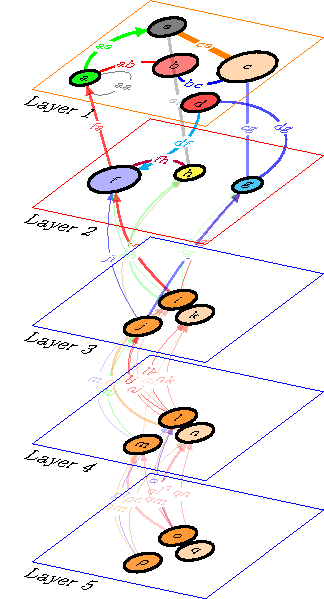
\includegraphics[width=9cm,height=14cm]{multilayer.pdf}\\
\end{center}
\caption{A five layer research platform: Data Integration (Layer 1),
  Complexity reduction (Layer 2), Pattern-process inference (Layer 3),
  Validation (Layer 4) and Visualization (Layer 5). Research platforms
  might play a leading role in accounting for bias and reproducibility
  in the pattern-process detection enterprise. a) A fully connected
  5-layer research platform, and b) A specific path representing the
  best solution to solve a task.}
\label{}
\end{figure}
  
\newpage
%The 5 layers described 
\begin{figure}
\begin{center}
\hspace{-0.5 in}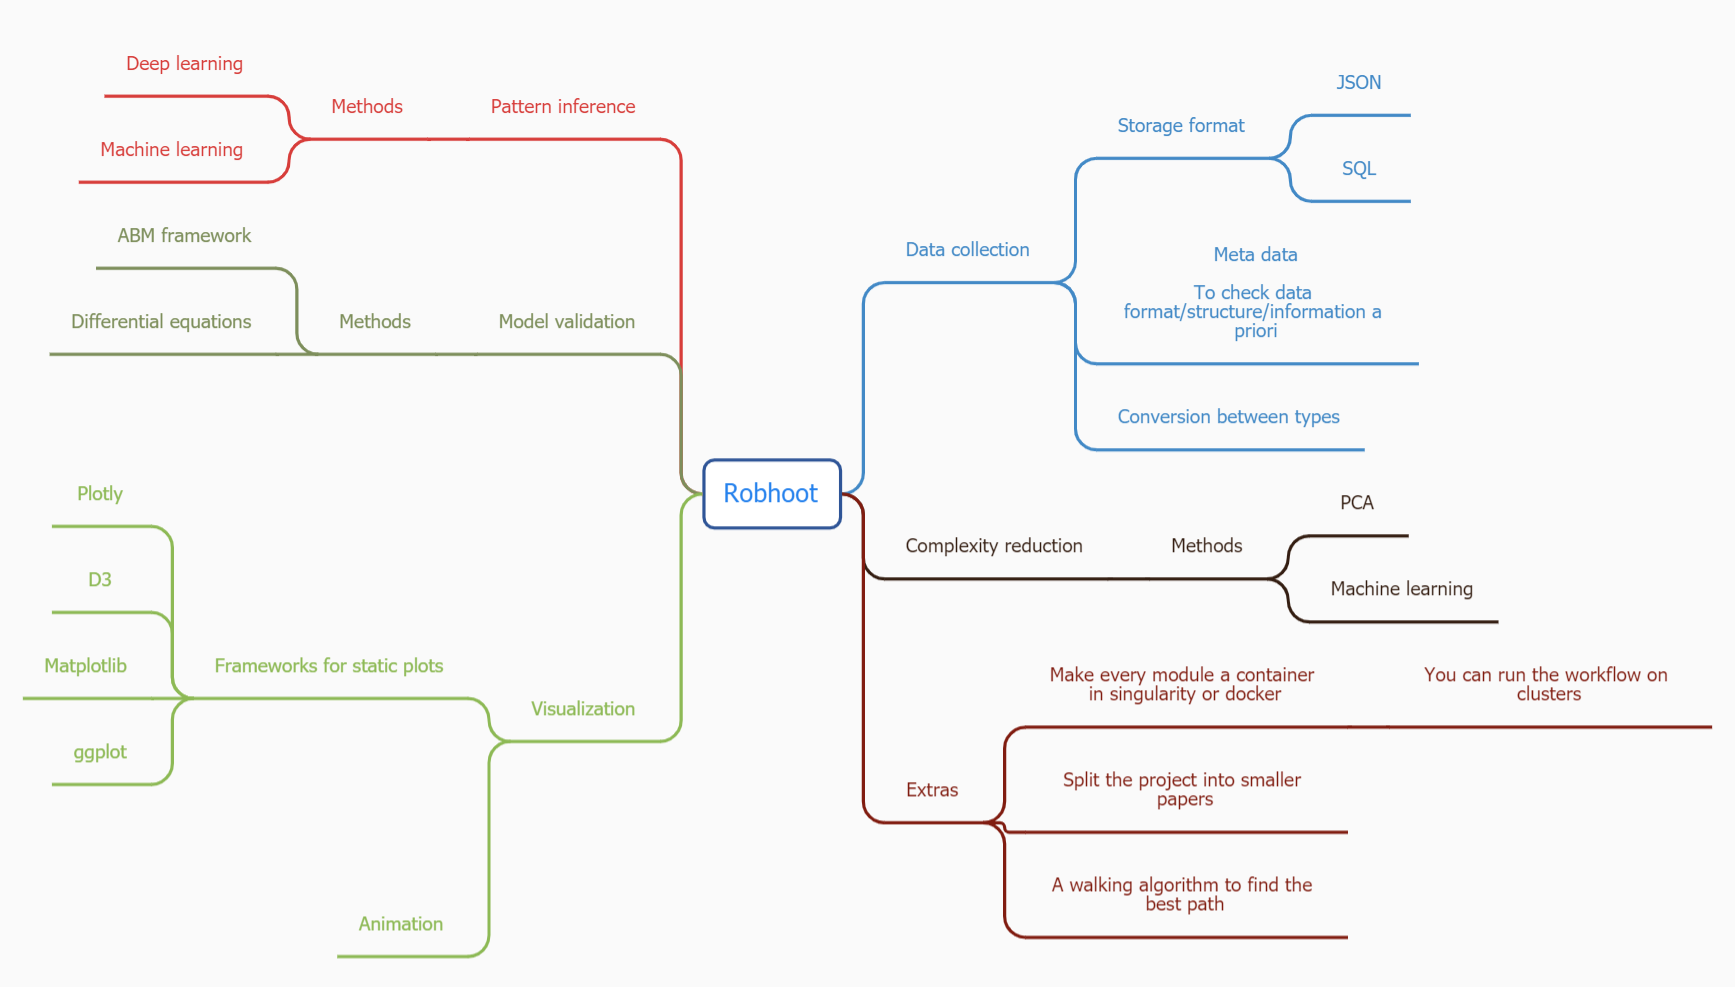
\includegraphics[scale=0.3,angle=90]{mindmap.png}
\end{center}
\caption{A mind map outlining the different methods to be used within each layer.}
\label{}
\end{figure}

\newpage
\begin{figure}
\begin{center}
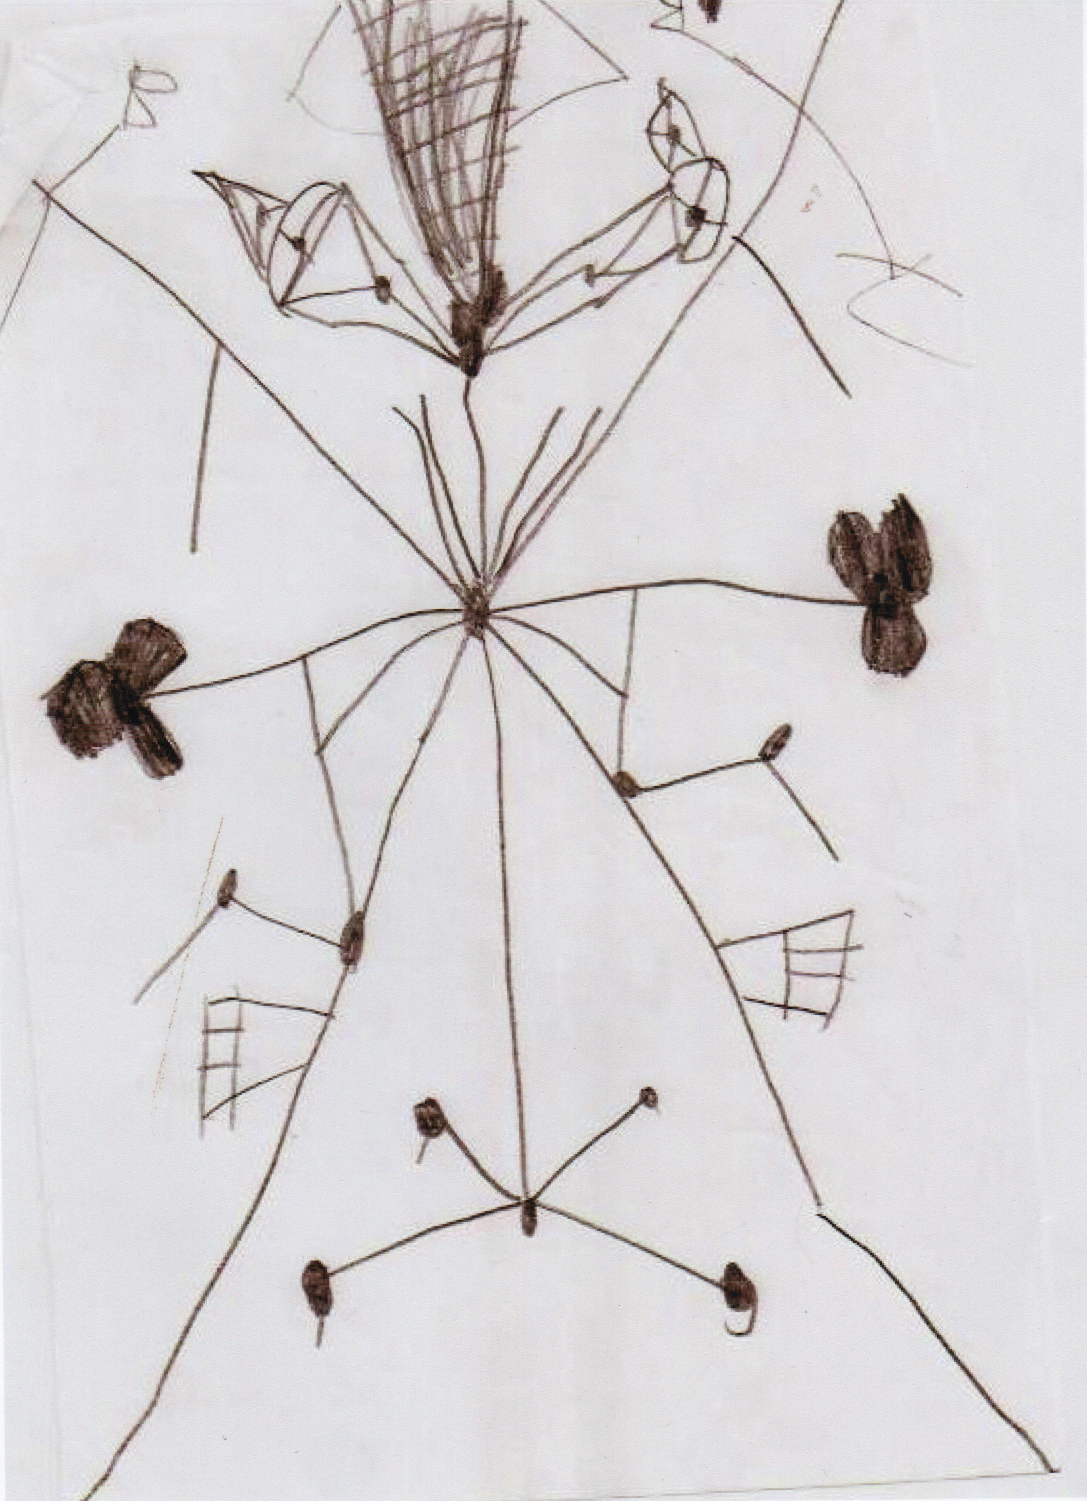
\includegraphics[scale=0.4]{robhootcartoon.pdf}
\end{center}
\caption{$\mathcal{ROBHOOT}$} -- An open multilayer platform for data integration, inference and prediction}
\end{figure}
\newpage



\newpage

%\begin{figure}
%\vspace{-1 in}
%\begin{center}
%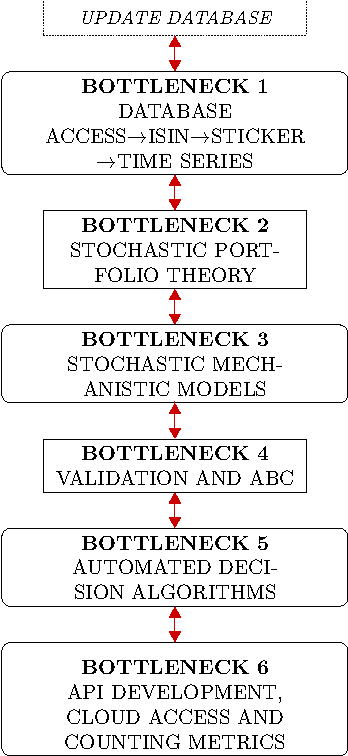
\includegraphics[scale=1.25]{EasyFlowChartBottlenecks.pdf}
%\end{center}
%\caption{Packages graph in $\mathcal{ROBHOOT}$: Visualization: Julia(Tikz and Tikz-network)}
%\end{figure}
%\newpage


\printindex
\end{document}
